\chapter{RQ2: Composing versus Transcribing}
\label{ch:rq2}
\section{Setup}
Replicate the Nosi scribing measure \cite{lueder2026nosi}: L-scale of
$\log(\mathrm{IAT})$ after removing pauses over 5 minutes and zero-length
intervals, classified with a linear SVM under leave-one-participant-out
cross-validation. Nosi's evidence is $N = 5$ expert authors on one task.
On simulated typists the recipe is tested as a classifier, since copying is known
there. Classroom data has no copying labels, so there the question is agreement with
weak signs (\cref{sec:weak-labels}): whether the L-scale and the process-channel score
are higher in windows before a big paste, a blocked outside paste, a paste after looking
away or keyless text than in the same student's other windows, and how strongly they
rank sessions with such signs first. Pasting one's own code produces the same signs, so
agreement is the claim, not accuracy.
\todo{Window length sweep (Nosi reports about 80\% at \SI{150}{\second});
comments-only typing as a known confound; per-student vs.\ population
thresholds.}
\section{Results}
\subsection*{Synthetic test students (evaluation harness)}
On the 36 synthetic test students (\cref{tab:harness-rq2,fig:harness-rq2}) the
Nosi recipe reaches 78\% balanced accuracy at 150\,s windows (interval 73--84\%),
close to the about 80\% Nosi reports; its accuracy peaks around 150\,s and falls
at 300\,s. Scoring the same L-scale against the student's own baseline instead
of one population threshold raises it to 91\%, and the process channel (pauses,
revisions, build order, runs, looking away) to 94\%, with both still improving
at longer windows. The per-student baseline, not a richer classifier, is what
helps the rhythm measure most.

With only five participants, as in Nosi's study, the same recipe gives 73\%
on average but anywhere from 51\% to 91\% depending on which five (5--95th
percentile over 200 random draws), so an $N=5$ result cannot distinguish a
good measure from a weak one; the personal and process scorers stay above 79\%
and 82\%.

\paragraph{Comments.} Chunks of 60 comment keystrokes from honest sessions are
judged ``transcribing'' by the code-trained threshold 37\% of the time, against
26\% for composed code and 71\% for transcribed code. In simulated data comments
differ from code only by a latency offset and fewer word pauses, so this is a
lower bound on the confound the study should expect.

% Generated by studentide.harness (synthetic:synth-v1-n120-s2026-b8-m30, test split, 36 students). Do not edit by hand.
\begin{table}[ht]
  \centering\small
  \caption{RQ2: composing vs.\ transcribing (condition D) per window, leave-one-participant-out balanced accuracy with 95\% bootstrap intervals over participants (synthetic test students). Nosi reports about 80\% at 150\,s with $N=5$.}
  \label{tab:harness-rq2}
  \resizebox{\linewidth}{!}{\begin{tabular}{@{}rccc@{}}
    \toprule
    $W$ (s) & Nosi L-scale & L-scale vs.\ own baseline & Process channel \\
    \midrule
    30 & 72\% {\scriptsize[69, 76]} & 79\% {\scriptsize[77, 81]} & 87\% {\scriptsize[86, 89]} \\
    60 & 74\% {\scriptsize[70, 79]} & 86\% {\scriptsize[83, 87]} & 91\% {\scriptsize[88, 93]} \\
    90 & 75\% {\scriptsize[71, 81]} & 88\% {\scriptsize[86, 91]} & 91\% {\scriptsize[88, 93]} \\
    120 & 77\% {\scriptsize[71, 84]} & 88\% {\scriptsize[85, 90]} & 94\% {\scriptsize[92, 95]} \\
    150 & 78\% {\scriptsize[73, 84]} & 91\% {\scriptsize[88, 93]} & 94\% {\scriptsize[90, 95]} \\
    300 & 71\% {\scriptsize[66, 79]} & 93\% {\scriptsize[89, 96]} & 96\% {\scriptsize[94, 97]} \\
    \midrule
    150, $N=5$ & 73\% {\scriptsize[51, 91]} & 88\% {\scriptsize[79, 95]} & 89\% {\scriptsize[82, 98]} \\
    \bottomrule
  \end{tabular}}
\end{table}


\begin{figure}[ht]
  \centering
  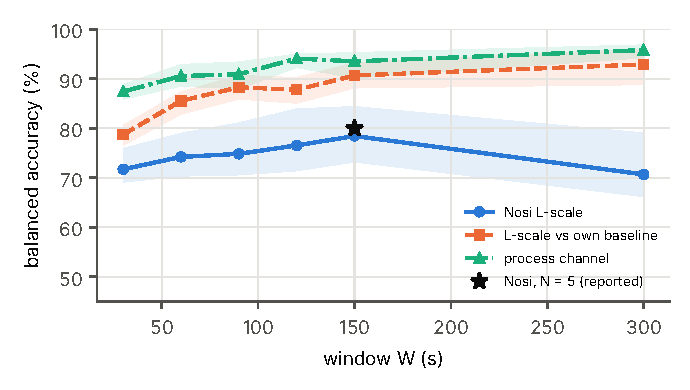
\includegraphics[width=0.65\linewidth]{harness-rq2}
  \caption{Composing vs.\ transcribing by window length (synthetic test students,
    95\% intervals over participants).}
  \label{fig:harness-rq2}
\end{figure}

\section{Summary}
